\documentclass[10pt,twocolumn]{article}
\usepackage[a4paper,margin=0.62in,top=0.68in,bottom=0.68in,columnsep=0.22in]{geometry}
\usepackage[utf8]{inputenc}
\usepackage[T1]{fontenc}
\usepackage{mathptmx}
\usepackage{graphicx}
\usepackage{booktabs}
\usepackage{amsmath,amssymb}
\usepackage{caption}
\usepackage{float}
\usepackage{hyperref}
\usepackage{xcolor}
\usepackage{enumitem}
\usepackage{titlesec}
\usepackage{fancyhdr}
\usepackage{multirow}
\usepackage{array}
\usepackage{dblfloatfix}

\setlength{\parskip}{3pt plus 1pt minus 1pt}
\setlength{\parindent}{0.8em}
\titlespacing*{\section}{0pt}{8pt}{4pt}
\titlespacing*{\subsection}{0pt}{6pt}{3pt}
\titleformat{\section}{\normalfont\large\bfseries}{\thesection.}{0.5em}{}
\titleformat{\subsection}{\normalfont\normalsize\bfseries}{\thesubsection}{0.5em}{}
\setlist{nosep,leftmargin=1.2em}
\captionsetup{font=small,labelfont=bf,skip=4pt}

\pagestyle{fancy}
\fancyhf{}
\renewcommand{\headrulewidth}{0.4pt}
\fancyhead[L]{\small RECS 2020 Electricity Regression}
\fancyhead[R]{\small RTSM Project}
\fancyfoot[C]{\small\thepage}

\hypersetup{colorlinks=true,linkcolor=blue!60!black,citecolor=blue!60!black,urlcolor=blue!60!black}

\begin{document}

\twocolumn[{%
\begin{center}
\vspace{0.3cm}
{\LARGE\bfseries Regression Analysis of U.S.\ Household\\[2pt] Annual Electricity Consumption}\\[10pt]
{\large Using the 2020 EIA Residential Energy Consumption Survey}\\[14pt]
{\normalsize\textit{Submitted for Regression and Time Series Models (MA60056)}}\\[4pt]
{\normalsize Submitted to: \textbf{Dr.\ Buddhananda Banerjee}}\\[10pt]
{\normalsize
\textbf{Team Members:}\\[6pt]
\renewcommand{\arraystretch}{1.2} % Adds a little breathing room between the names and roll numbers
\begin{tabular}{ccccc}
Anmol Gulati & Pranav Taneja & Prateek Hegde & Sneha Yadav & Vybhav Chaturvedi \\
25BM6JP04 & 25BM6JP37 & 25BM6JP39 & 25BM6JP49 & 25BM6JP60 \\
\end{tabular}
}\\[10pt]
{\small
\textbf{GitHub:} \url{https://github.com/vybhav72954/household_electricity}\\[2pt]
\textbf{Google Drive:} \url{https://drive.google.com/drive/u/2/folders/1p8gR59MZd-9KokQtJyjXErHQvd-1BbWK}
}\\[4pt]
\rule{0.6\textwidth}{0.5pt}
\vspace{0.4cm}
\end{center}
}]

% ════════════════════════════════════════════════════════════
\section{Introduction}

Understanding the determinants of household electricity consumption is central to energy policy, utility demand forecasting, and residential carbon mitigation. As the electrification of heating, transportation, and cooking accelerates, quantifying the structural and behavioural drivers of residential electricity use becomes increasingly important for grid planning and rate design.

This report presents an end-to-end regression analysis of annual household electricity consumption (KWH) using the 2020 Residential Energy Consumption Survey (RECS) microdata published by the U.S.\ Energy Information Administration (EIA). RECS is the most comprehensive nationally representative survey of U.S.\ residential energy use, covering dwelling characteristics, appliance inventories, occupant demographics, thermostat behaviour, climate zones, and metered energy consumption outcomes.

The analysis proceeds through five stages: (1)~data inspection and cleaning, (2)~exploratory data analysis, (3)~multicollinearity diagnostics and feature selection, (4)~OLS model specification with robust inference, and (5)~benchmarking against regularised and tree-based models. Our primary goals are:

\begin{itemize}
\item Identify the dominant household-level drivers of electricity consumption using an interpretable OLS model with heteroskedasticity-robust standard errors.
\item Benchmark predictive performance across linear, regularised, and gradient-boosted models on both log-transformed and original KWH scales.
\item Evaluate whether engineered composite features (e.g., electronics load proxy, space per person) add explanatory power beyond raw survey fields.
\end{itemize}

% ════════════════════════════════════════════════════════════
\section{Data Description}

\subsection{Dataset Overview}

The raw RECS 2020 file comprises 18{,}496 surveyed households and 799 variables. Only 10 columns contain any missing values (all related to electric vehicle charging), and there are zero duplicate rows. The dataset includes 61 survey weight columns (\texttt{NWEIGHT}, \texttt{NWEIGHT1}--\texttt{NWEIGHT60}) for population-level inference; our modelling uses unweighted estimation, retaining weights as metadata only. Table~\ref{tab:summary} presents summary statistics for the target and key numeric features.

\begin{table}[H]
\centering
\caption{Summary statistics for target and key features ($n = 18{,}496$).}
\label{tab:summary}
\small
\setlength{\tabcolsep}{3pt}
\begin{tabular}{@{}lrrrrr@{}}
\toprule
\textbf{Variable} & \textbf{Mean} & \textbf{SD} & \textbf{Median} & \textbf{Min} & \textbf{Max}\\
\midrule
KWH (annual)        & 10{,}632 & 7{,}071 & 8{,}944 & 473 & 108{,}327\\
log1p(KWH)          & 9.03 & 0.67 & 9.10 & 6.16 & 11.59\\
Conditioned sqft    & 1{,}753 & 1{,}084 & 1{,}500 & 100 & 13{,}000\\
Household size      & 2.53 & 1.37 & 2 & 1 & 14\\
CDD (30yr)          & 1{,}249 & 859 & 1{,}042 & 0 & 5{,}095\\
Num.\ refrigerators & 1.19 & 0.47 & 1 & 0 & 6\\
Num.\ freezers      & 0.37 & 0.53 & 0 & 0 & 6\\
\bottomrule
\end{tabular}
\end{table}

\subsection{Column Selection and Leakage Prevention}

From the 799 columns, we selected 73 raw fields across nine conceptual groups (Table~\ref{tab:groups}). Three outcome-adjacent fields were explicitly excluded as leakage risks: annual electricity spend (\texttt{DOLLAREL}), total site BTU (\texttt{TOTALBTU}), and total energy spend (\texttt{TOTALDOL}). These are direct transformations or near-deterministic functions of the target and would artificially inflate $R^2$.

\begin{table}[H]
\centering
\caption{Column groups used in the analysis.}
\label{tab:groups}
\footnotesize
\setlength{\tabcolsep}{3pt}
\begin{tabular}{@{}llc@{}}
\toprule
\textbf{Group} & \textbf{Examples} & \textbf{$n$}\\
\midrule
Identifiers / Weights & DOEID, NWEIGHT, REGIONC & 4\\
Climate \& Geography & BA\_climate, CDD30YR, HDD30YR & 4\\
Dwelling Structure   & TYPEHUQ, KOWNRENT, STORIES & 4\\
Size \& Vintage      & TOTSQFT\_EN, BEDROOMS, SQFTEST & 9\\
Equipment / Systems  & AIRCOND, NUMFRIG, SWIMPOOL & 14\\
Household Behaviour  & TEMPHOME, WASHLOAD & 16\\
Electronics          & TVCOLOR, DESKTOP & 13\\
Household Comp.      & NHSLDMEM, HHAGE, MONEYPY & 8\\
Fuel Types           & ALLELEC, USENG, USELP & 5\\
\midrule
\multicolumn{2}{@{}l}{Outcomes (kept for target only)} & 4\\
\bottomrule
\end{tabular}
\end{table}

\subsection{Target Selection}

The candidate target variables were KWH (annual electricity consumption), log1p(KWH), DOLLAREL (annual spend), and TOTALBTU (total site energy). Raw KWH exhibits strong right skew (1.83), driven by a long tail of high-consumption households exceeding 40{,}000~KWH/year. Table~\ref{tab:targets} compares all four candidates. Applying $y = \log(1 + \text{KWH})$ reduces skew to $-0.44$, producing a near-symmetric distribution suitable for OLS assumptions (Figure~\ref{fig:target}). DOLLAREL was excluded as outcome-adjacent, and TOTALBTU was excluded as a multi-fuel composite that introduces leakage from non-electric energy sources.

\begin{table}[H]
\centering
\caption{Candidate target comparison.}
\label{tab:targets}
\small
\begin{tabular}{@{}llr@{}}
\toprule
\textbf{Candidate} & \textbf{Rationale} & \textbf{Skew}\\
\midrule
KWH         & Direct outcome              & 1.83\\
log1p(KWH)  & Variance-stabilised target  & $-$0.44\\
DOLLAREL     & Outcome-adjacent (leakage) & 2.13\\
TOTALBTU     & Multi-fuel leakage risk    & 2.72\\
\bottomrule
\end{tabular}
\end{table}

\begin{figure}[H]
\centering
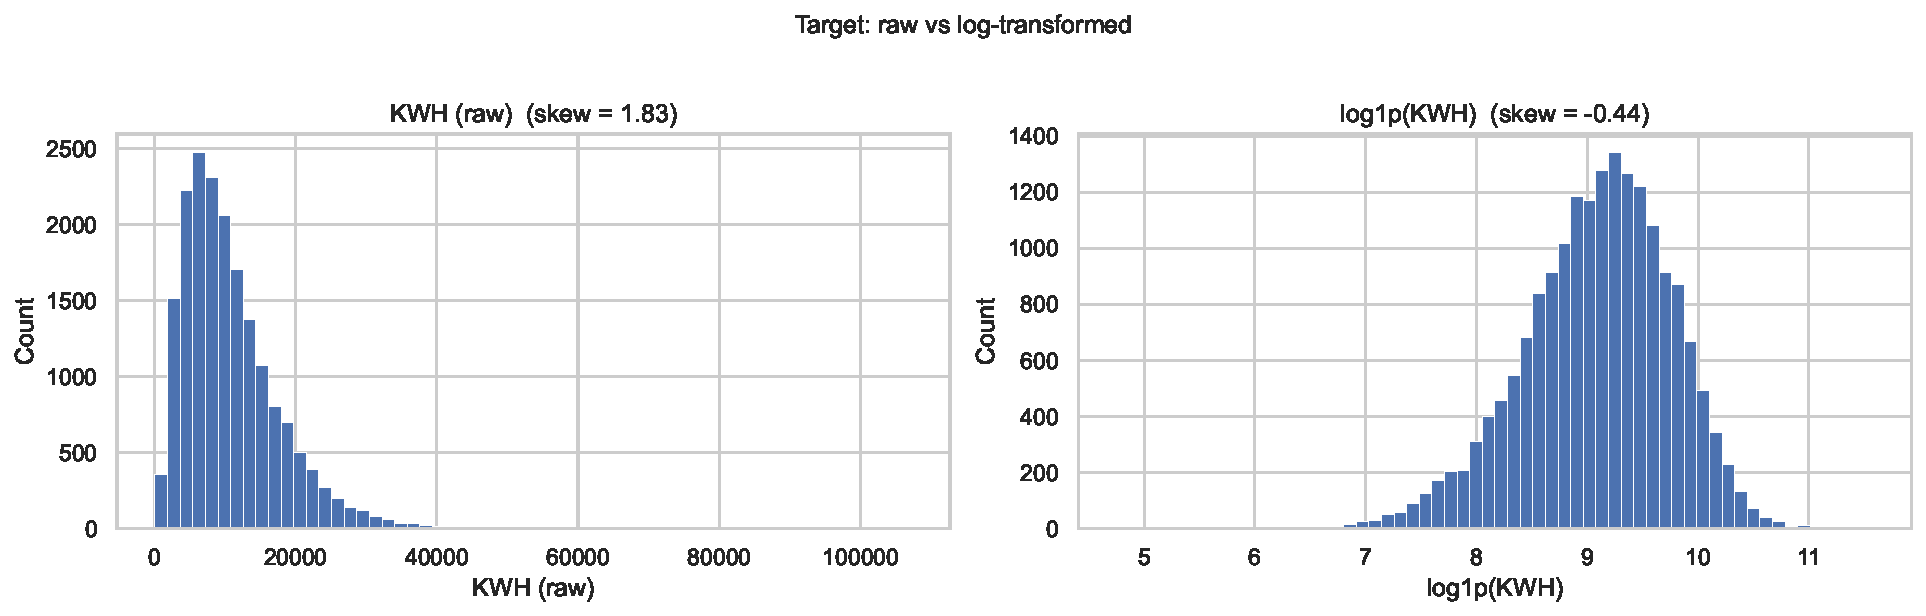
\includegraphics[width=\linewidth]{raw_vs_log-transform.pdf}
\caption{Target distribution: raw KWH (skew~=~1.83) vs.\ log1p(KWH) (skew~=~$-$0.44). The log transform substantially reduces right skew.}
\label{fig:target}
\end{figure}

Figure~\ref{fig:target_kde} shows the same distributions with kernel density estimation overlaid, confirming that the log-transformed target closely approximates a Gaussian (with mild left skew).

\begin{figure}[H]
\centering
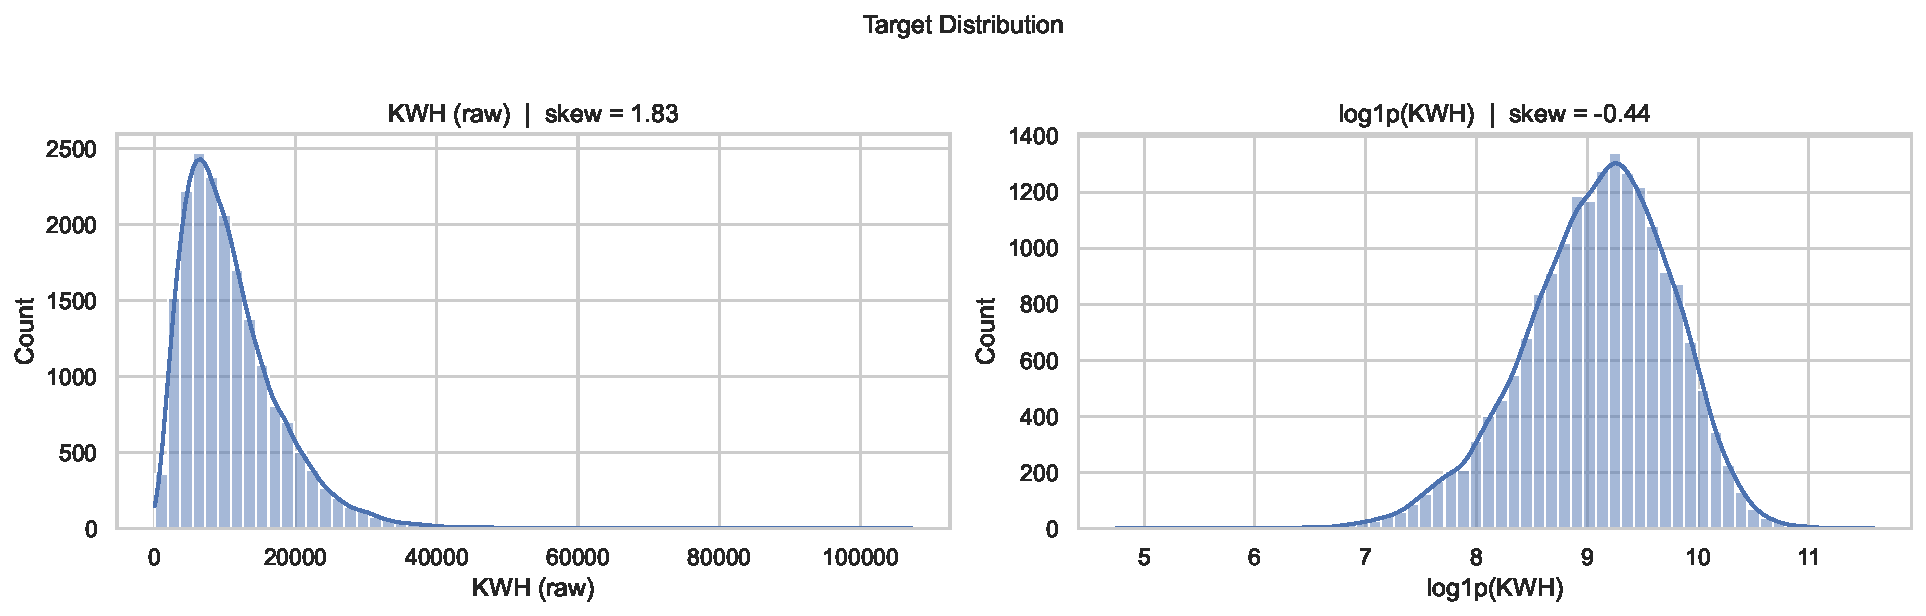
\includegraphics[width=\linewidth]{target_distribution.pdf}
\caption{Target distributions with KDE overlay. The log1p(KWH) distribution is approximately normal with a slight left tail.}
\label{fig:target_kde}
\end{figure}

\subsection{Cleaning and Feature Engineering}

RECS uses special codes to indicate missing or inapplicable responses: $-2$ (not applicable), $-1$ (missing), and 97--99 (refused / don't know). Thermostat fields (\texttt{TEMPHOME}, \texttt{TEMPGONE}, \texttt{TEMPNITE} and their summer equivalents) additionally use 997--999 as special codes. All such codes were replaced with NaN before analysis.

Categorical codes were mapped to readable labels (e.g., \texttt{TYPEHUQ} $1 \rightarrow$ ``Mobile home'', $2 \rightarrow$ ``Single-family detached''). Six engineered features were created:

\begin{itemize}
\item \texttt{log\_conditioned\_sqft}: $\log(1 + \text{sqft})$, linearising the size--consumption relationship.
\item \texttt{sqft\_per\_person}: conditioned area per household member---a density proxy.
\item \texttt{ac\_unit\_count}: sum of ductless, window/wall, and portable AC units.
\item \texttt{electronics\_load\_proxy}: aggregate count of TVs, streaming devices, game consoles, audio systems, desktops, laptops, tablets, and smartphones.
\item \texttt{children\_share}: proportion of household members who are children.
\item \texttt{summer\_setpoint\_spread}: thermostat away minus home daytime temperature---a setback behaviour proxy.
\end{itemize}

After cleaning, the working dataframe contains 18{,}496 rows and 99 columns. The data were split 80/20 (14{,}796 train, 3{,}700 test), stratified by census region for balanced geographic representation.

% ════════════════════════════════════════════════════════════
\section{Exploratory Data Analysis}

\subsection{Climate and Housing Type}

Figure~\ref{fig:climate_housing} reveals that Hot-Humid climates (predominantly the U.S.\ Southeast) have the highest median KWH at ${\sim}$13{,}000, roughly double the Subarctic median of ${\sim}$6{,}500. This reflects sustained cooling loads driven by prolonged high temperatures and humidity. Among housing types, mobile homes consume the most (median ${\sim}$11{,}000~KWH), likely due to poorer thermal envelopes and smaller shared-wall area, while Apartment 5+ units consume the least (${\sim}$5{,}000~KWH), reflecting smaller floor areas and shared-wall insulation benefits.

\begin{figure}[H]
\centering
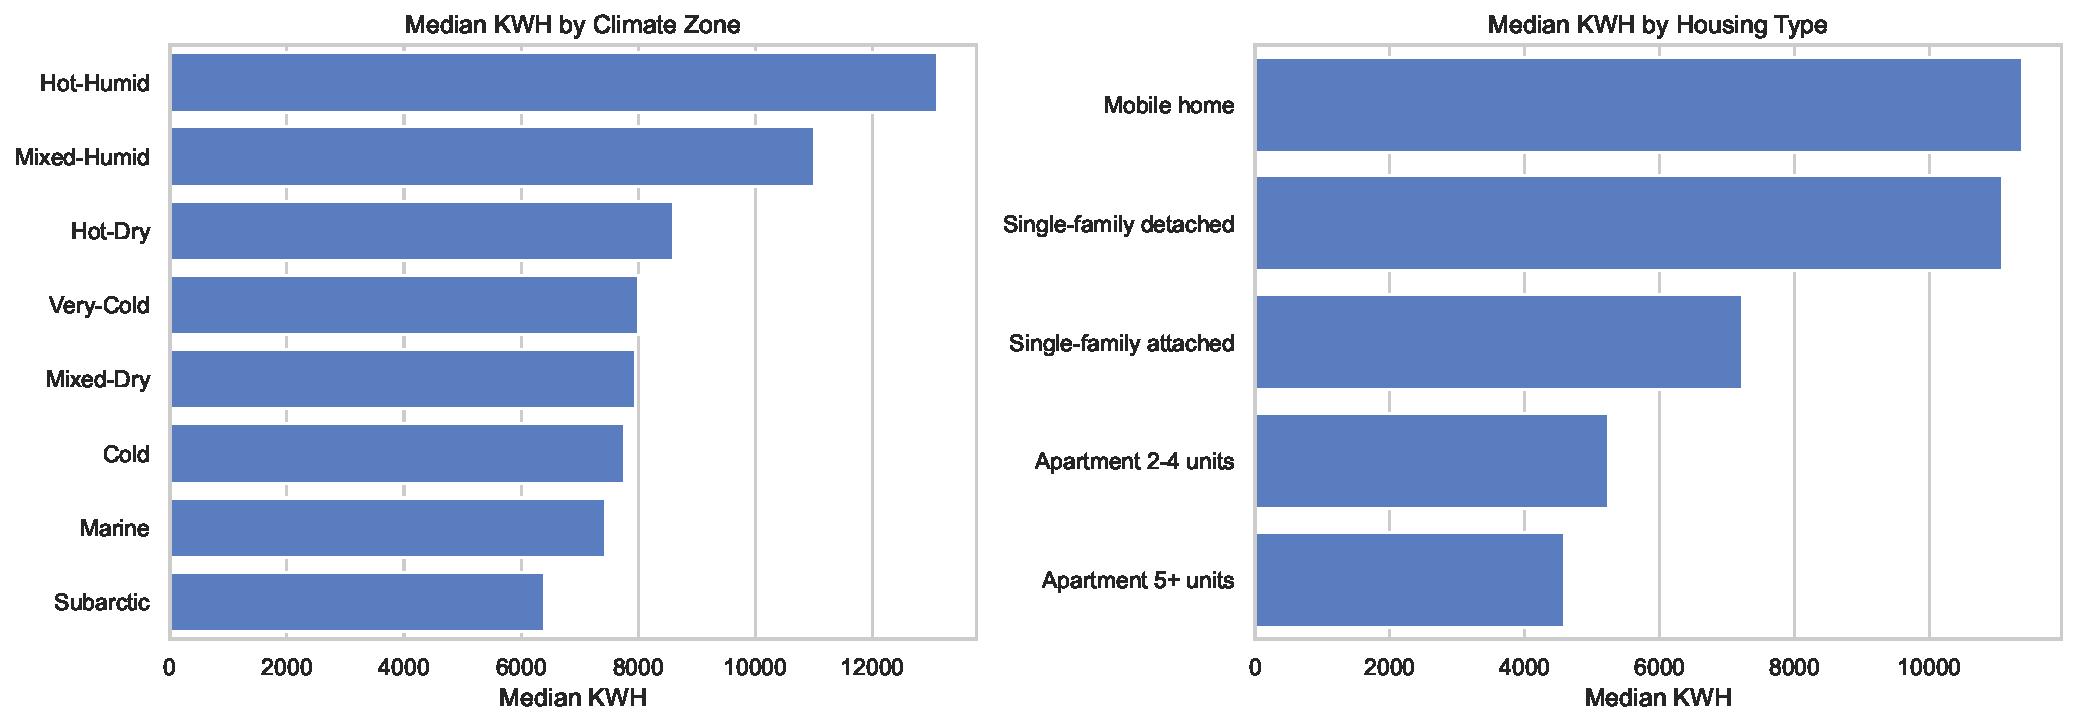
\includegraphics[width=\linewidth]{KWH_by_climate_zone_housing_type.pdf}
\caption{Median annual KWH by climate zone and housing type.}
\label{fig:climate_housing}
\end{figure}

\subsection{Equipment and Occupancy Effects}

Figure~\ref{fig:equipment} confirms that electricity use scales monotonically with household size, increasing from a median of ${\sim}$7{,}500~KWH for single-person households to ${\sim}$16{,}000 for households of seven. Air conditioning raises the median by roughly 4{,}000~KWH. All-electric homes show a particularly large uplift: their median (${\sim}$13{,}000~KWH) is nearly double that of non-all-electric homes (${\sim}$7{,}500~KWH), reflecting the substitution of gas heating, water heating, and cooking with electric equivalents.

\begin{figure}[H]
\centering
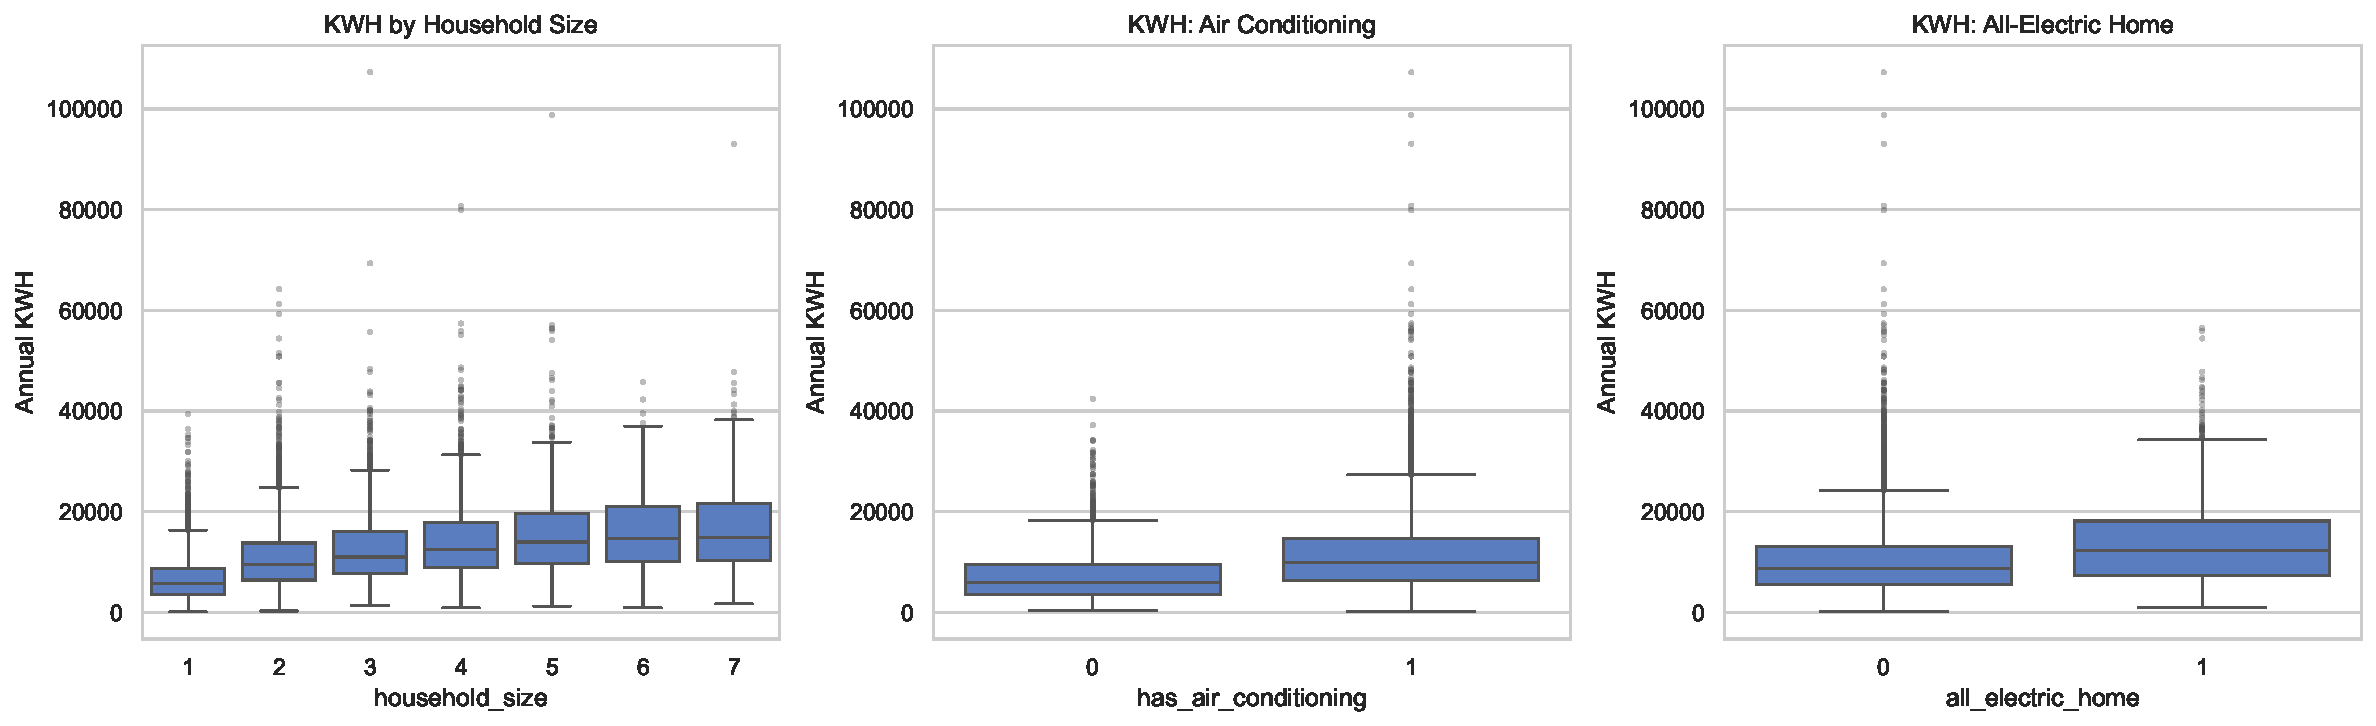
\includegraphics[width=\linewidth]{Occupancy_equipment_box_plots.pdf}
\caption{KWH distributions by household size, AC status, and all-electric status.}
\label{fig:equipment}
\end{figure}

\subsection{Size--Consumption Relationship}

The scatter of KWH against conditioned square footage (Figure~\ref{fig:scatter}) shows a positive but heteroskedastic relationship. The variance of KWH increases with dwelling size, and Hot-Humid households (purple) sit consistently above the point cloud, confirming the joint effect of climate and size. This pattern motivates using log-transformed size alongside climate zone dummies as joint predictors, and justifies the log target transform for variance stabilisation.

\begin{figure}[H]
\centering
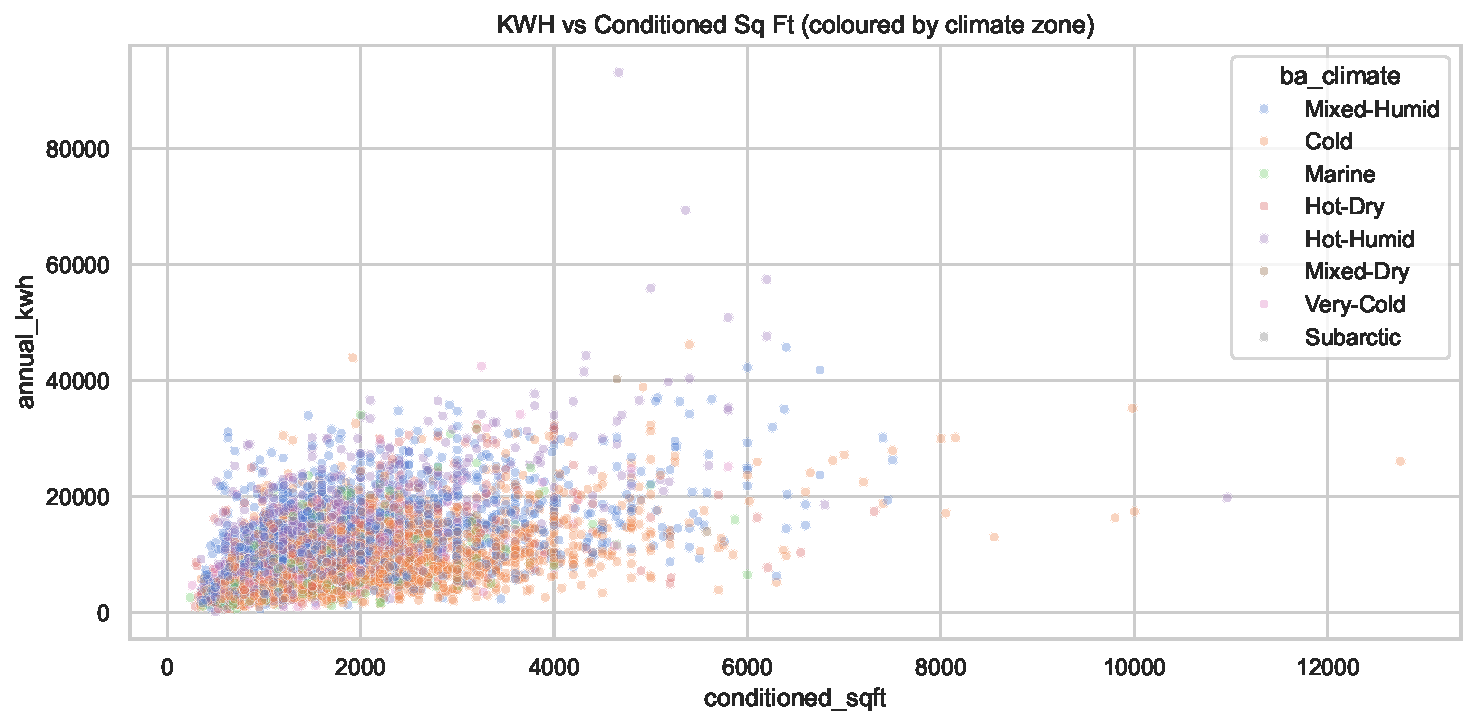
\includegraphics[width=\linewidth]{KWH_vs_square_footage_coloured_by_climate.pdf}
\caption{KWH vs.\ conditioned sq.\ ft., coloured by climate zone. Hot-Humid (purple) and Mixed-Humid (blue) points dominate the upper portion of the cloud.}
\label{fig:scatter}
\end{figure}

\subsection{Geographic Variation}

The top-consuming states---Louisiana, Mississippi, Florida, Alabama, Tennessee---are all in the Southeast, reflecting high cooling loads and prevalence of all-electric homes (Figure~\ref{fig:geo}). Low-consumption states---California, District of Columbia, New York, Alaska---combine mild climates or dense housing stock with lower electric heating reliance. The geographic pattern aligns closely with the climate zone findings and validates using climate zone as a modelling feature rather than state fixed effects (which would be less parsimonious).

\begin{figure}[H]
\centering
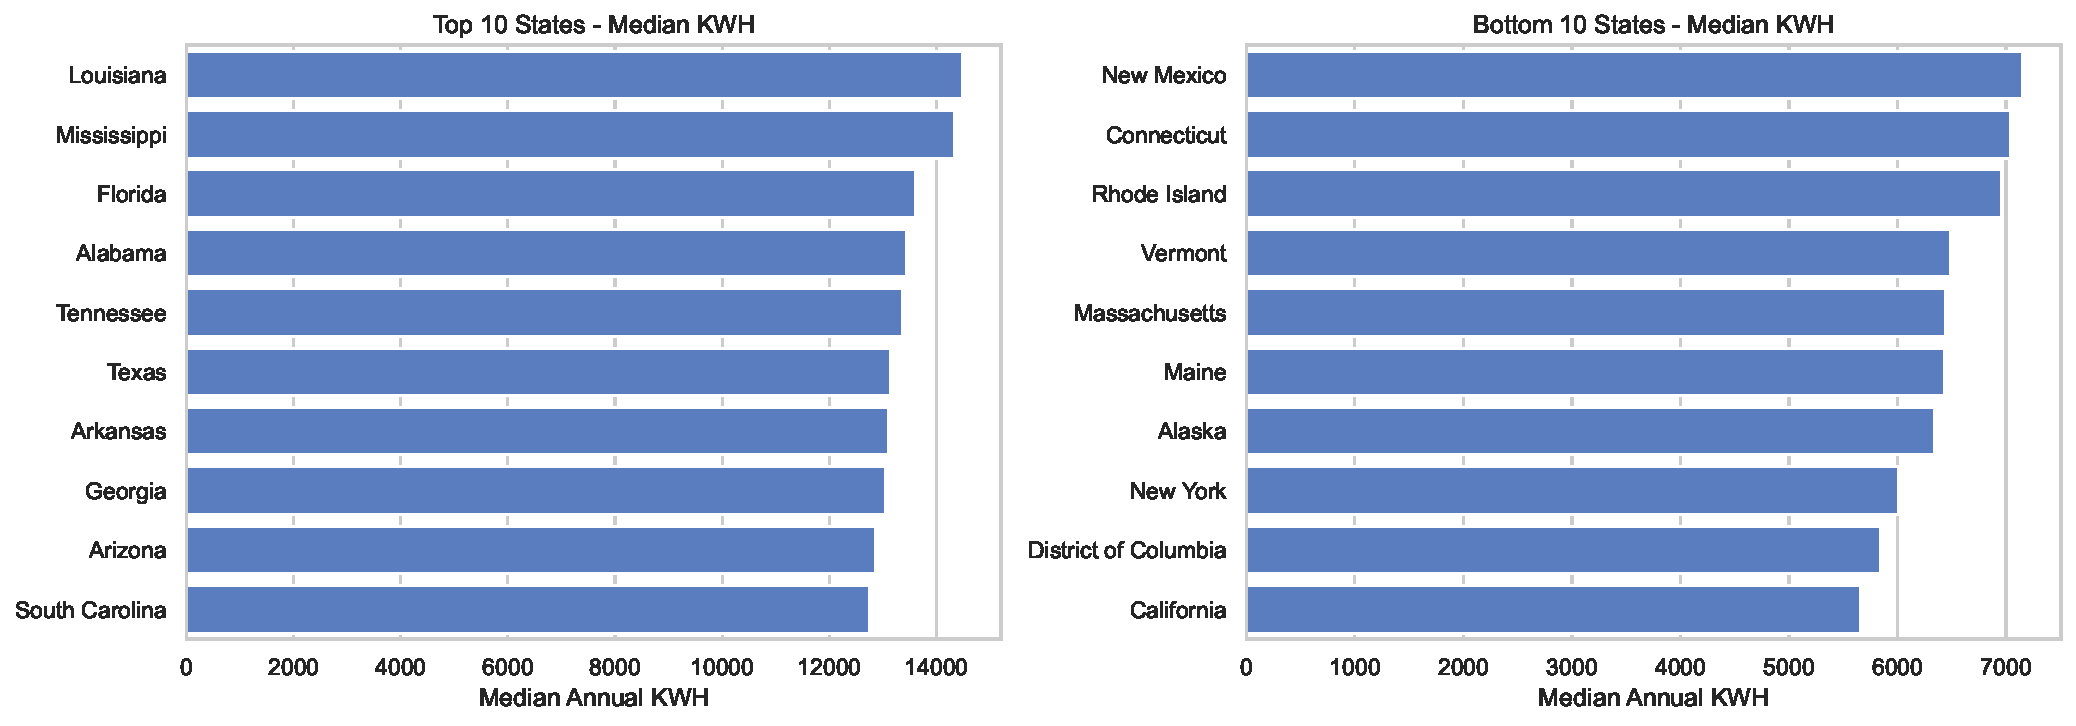
\includegraphics[width=\linewidth]{Geographic_variation.pdf}
\caption{Top and bottom 10 states by median annual KWH.}
\label{fig:geo}
\end{figure}

\subsection{Thermostat Behaviour}

After correcting for RECS special codes (997--999), thermostat setpoints cluster tightly around 68--72\textdegree F for both summer and winter (Figure~\ref{fig:thermo}). There is no strong linear relationship between setpoint level and KWH---the scatter is diffuse, and extremes in both directions show similar KWH ranges. This suggests that setpoint behaviour operates at the margin: it matters conditional on climate and dwelling type, but it is not a dominant univariate predictor. The engineered \texttt{summer\_setpoint\_spread} feature captures the behavioural signal (setback discipline) more effectively than the raw setpoint level.

\begin{figure}[H]
\centering
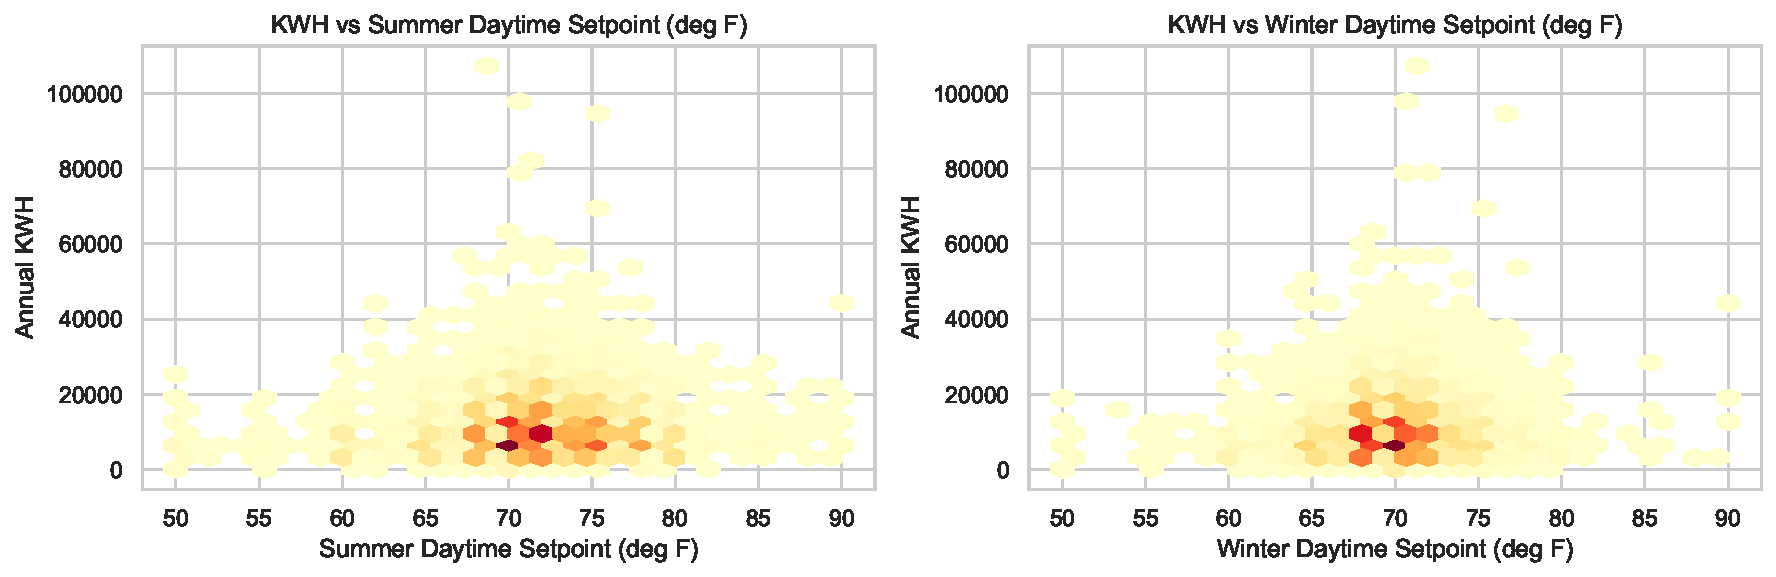
\includegraphics[width=\linewidth]{Thermostat_setpoint_vs_KWH.pdf}
\caption{KWH vs.\ summer (left) and winter (right) daytime thermostat setpoints (\textdegree F). Density concentrated at 68--72\textdegree F with no clear linear trend.}
\label{fig:thermo}
\end{figure}

\subsection{Numeric Feature Correlations}

Among the numeric features retained for modelling, \texttt{log\_conditioned\_sqft} shows the strongest Pearson correlation with log1p(KWH) at $r = 0.51$, followed by \texttt{full\_bathrooms} ($0.47$), \texttt{electronics\_load\_proxy} ($0.45$), \texttt{household\_size} ($0.40$), \texttt{num\_refrigerators} ($0.40$), and \texttt{num\_freezers} ($0.30$) (Figure~\ref{fig:corr_target}). Notably, \texttt{sqft\_per\_person} has only marginal univariate correlation ($0.07$) but may still contribute conditional on other features, since it captures the interaction of size and occupancy.

\begin{figure}[H]
\centering
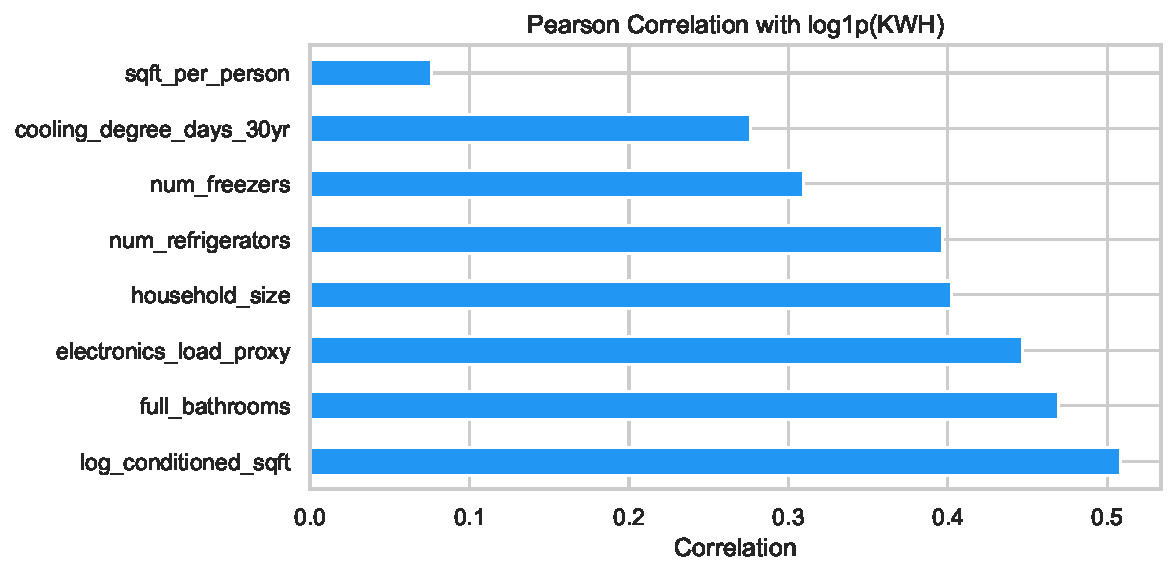
\includegraphics[width=\linewidth]{Correlation_with_log_target.pdf}
\caption{Pearson correlation of numeric features with log1p(KWH).}
\label{fig:corr_target}
\end{figure}

% ════════════════════════════════════════════════════════════
\section{Methodology}

\subsection{Modelling Framework}

The modelling workflow consists of four phases: (a)~OLS baseline with robust inference, (b)~multicollinearity diagnostics and pruning, (c)~regularised linear models, and (d)~gradient-boosted regression. All models predict $y = \log(1 + \text{KWH})$ using the same train/test split (80/20, stratified by census region). Performance is evaluated on both the log scale (where fitting occurs) and the original KWH scale (obtained via $\hat{y}_{\text{KWH}} = e^{\hat{y}_{\log}} - 1$, where Jensen's inequality introduces a small negative bias that we accept for simplicity).

\subsection{Evaluation Metrics}

All models are assessed with five metrics reported on both scales:

\begin{itemize}
\item $R^2$: proportion of variance explained. Reported for both train and test; adjusted $R^2$ is reported for train only (it is not meaningful on held-out data).
\item RMSE (root mean squared error): emphasises large deviations.
\item MAE (mean absolute error): robust central-tendency measure.
\item MAPE (mean absolute percentage error): business-interpretable --- ``on average, the model's prediction is off by X\% of actual consumption.''
\end{itemize}

\subsection{Preprocessing}

Numeric features are imputed with median values (robust to skew and outliers). Binary features are imputed with the most frequent value. Categorical features are imputed with the most frequent category and then one-hot encoded with the first category dropped (to avoid perfect collinearity). For regularised models, numeric features are additionally standardised to zero mean and unit variance. OLS uses unstandardised inputs so that coefficients have direct unit interpretations.

\subsection{Baseline}

A naive mean baseline (predicting $\bar{y}_{\text{train}}$ for every observation) establishes the floor: any useful model must substantially exceed its test $R^2$ of approximately zero (and negative on the KWH scale due to Jensen's inequality on the back-transformation).

% ════════════════════════════════════════════════════════════
\section{Multicollinearity Diagnostics}

Before specifying the OLS model, we screened 16 numeric candidate features for multicollinearity using variance inflation factors (VIF). The initial candidate set exhibited severe collinearity among the size-related variables (Table~\ref{tab:vif}): \texttt{log\_conditioned\_sqft} had VIF~=~127, \texttt{conditioned\_sqft} had 82, and \texttt{heated\_sqft} had 67. These reflect the near-mechanical relationship between total, heated, and cooled floor area in RECS.

\begin{table}[H]
\centering
\caption{VIF before and after pruning.}
\label{tab:vif}
\small
\begin{tabular}{@{}lrr@{}}
\toprule
\textbf{Feature} & \textbf{Initial} & \textbf{Pruned}\\
\midrule
log\_conditioned\_sqft & 126.8 & 14.8 \\
conditioned\_sqft      &  82.3 & \textit{dropped}\\
heated\_sqft           &  67.2 & \textit{dropped}\\
heated\_share          &  54.3 & \textit{dropped}\\
total\_rooms           &  29.8 & \textit{dropped}\\
cooled\_share          &  27.1 & \textit{dropped}\\
bedrooms               &  26.2 & \textit{dropped}\\
cooled\_sqft           &  24.8 & \textit{dropped}\\
household\_size        &  22.8 & 11.9\\
full\_bathrooms        &  14.1 & 9.0\\
num\_refrigerators     & ---   & 6.5\\
num\_children          &   3.7 & 3.4\\
cooling\_degree\_days  &  15.6 & 2.7\\
num\_freezers          & ---   & 1.6\\
\bottomrule
\end{tabular}
\end{table}

The pruning strategy retained one representative per collinear cluster:

\begin{itemize}
\item \textbf{Dwelling size:} \texttt{log\_conditioned\_sqft} retained; raw area variants, heated/cooled sqft, bedrooms, total rooms, and area shares dropped.
\item \textbf{Layout:} \texttt{full\_bathrooms} retained (bedrooms and total\_rooms are collinear with sqft at $r > 0.6$).
\item \textbf{Occupancy:} \texttt{household\_size} + \texttt{num\_children} retained as distinct signals---size captures total load, while children captures the differential per-capita effect.
\item \textbf{Climate:} \texttt{cooling\_degree\_days} retained; heating degree days dropped (collinear at $r = 0.85$ with CDD via \texttt{cooling\_intensity\_proxy}).
\end{itemize}

Two features---\texttt{log\_conditioned\_sqft} (VIF~14.8) and \texttt{household\_size} (VIF~11.9)---remain slightly above the conventional VIF~=~10 threshold. Both are core predictors: removing either would substantially reduce explanatory power. Their retention is justified by substantive importance and the use of HC3 robust standard errors, which remain consistent under multicollinearity.

The correlation heatmap (Figure~\ref{fig:corr_heat}) confirms these decisions: the upper-left block of size-related variables shows correlations of 0.60--0.93, while the retained pruned features have manageable pairwise correlations.

\begin{figure}[H]
\centering
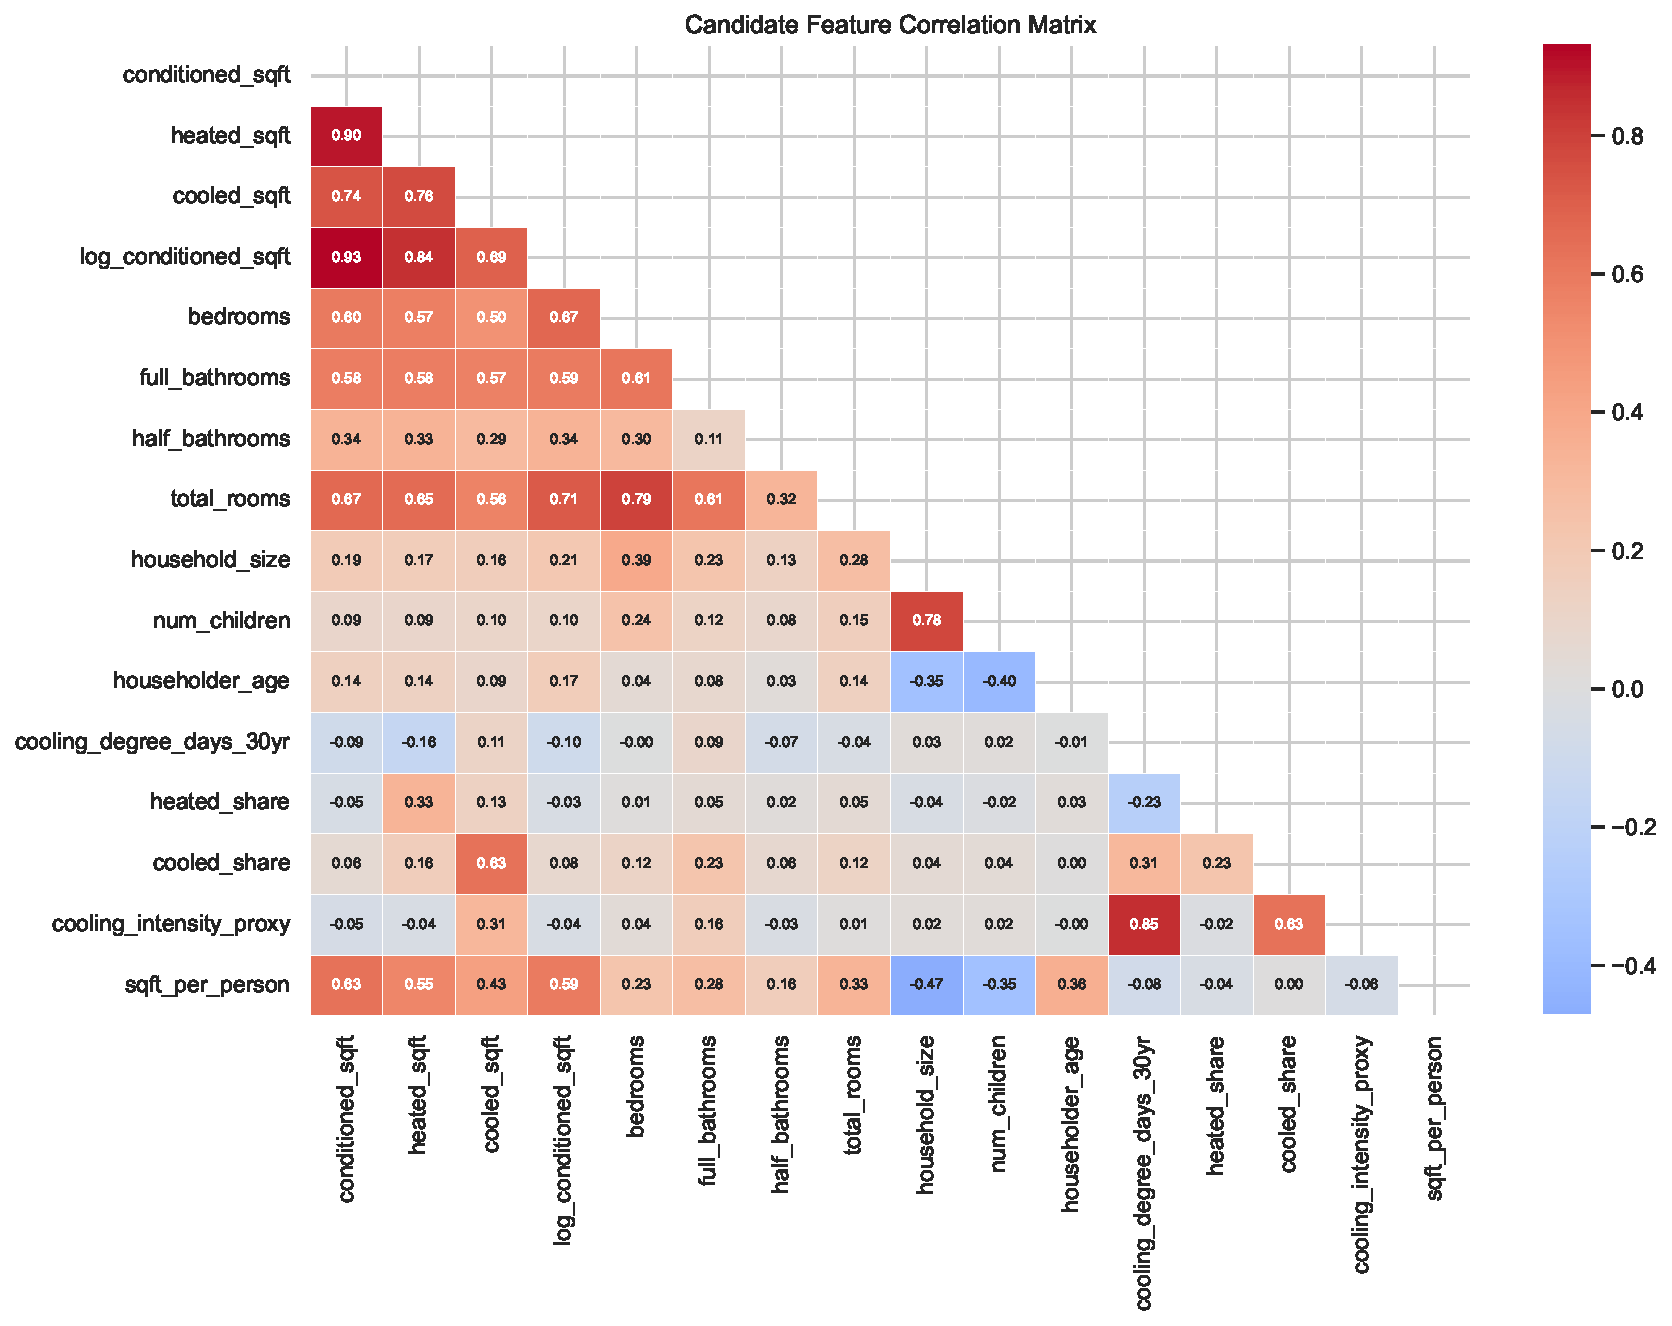
\includegraphics[width=\linewidth]{Correlation_heatmap.pdf}
\caption{Correlation matrix of 16 numeric candidate features. The size-related cluster (top-left) motivates aggressive pruning.}
\label{fig:corr_heat}
\end{figure}

% ════════════════════════════════════════════════════════════
\section{OLS Model Specification}

\subsection{Feature Sets}

Three feature sets were defined for use across models (Table~\ref{tab:fsets}). The OLS Candidate set was the wider starting point. The Expanded set dropped \texttt{householder\_age}, \texttt{uses\_propane}, \texttt{urbanicity\_band}, and \texttt{employment\_band}---all with weaker incremental contributions. The Engineered set extended the Expanded set with five derived features.

\begin{table}[H]
\centering
\caption{Feature sets used across models.}
\label{tab:fsets}
\small
\begin{tabular}{@{}lccc@{}}
\toprule
\textbf{Set} & \textbf{Numeric} & \textbf{Binary} & \textbf{Categorical}\\
\midrule
OLS Candidate & 8 & 6 & 5\\
Expanded (Pruned) & 7 & 5 & 3\\
Engineered & 11 & 5 & 3\\
\bottomrule
\end{tabular}
\end{table}

\subsection{Initial vs.\ Pruned OLS}

The initial OLS on the candidate set (33 regressors after one-hot encoding) achieved train/test $R^2$ of 0.708/0.703 on the log scale. After inspecting HC3 robust $p$-values, four groups were pruned:

\begin{itemize}
\item \texttt{urbanicity\_band}: weak incremental contribution beyond housing type and climate zone; most of its signal is absorbed by the dwelling structure and climate dummies.
\item \texttt{employment\_band}: weakly significant, and conceptually mediated through household size and income (which are already captured indirectly via dwelling size and appliance ownership).
\item \texttt{uses\_propane}: a niche fuel indicator affecting $<$5\% of households, with a small and unstable coefficient.
\item \texttt{householder\_age}: marginally significant ($t = -2.0$, $p = 0.043$) under HC3, and conceptually less direct than \texttt{household\_size} and \texttt{num\_children} as occupancy measures.
\end{itemize}

The pruned model (25 regressors) loses negligibly: 0.705/0.699. The AIC increases only marginally (11{,}840 $\rightarrow$ 11{,}980), and the BIC actually favours the pruned model due to the complexity penalty. This confirms the pruned specification is parsimonious without meaningful information loss.

\subsection{Pruned OLS Coefficients (HC3)}

All inference uses HC3 heteroskedasticity-robust standard errors, which are consistent under heteroskedasticity without requiring a specific variance model. Table~\ref{tab:ols} presents the complete coefficient table. All numeric and binary predictors are significant at $p < 0.001$. Among climate dummies (reference: Cold), Mixed-Humid ($t = 21.2$), Very-Cold ($t = 6.7$), and Marine ($t = 5.3$) are significant; Hot-Humid ($p = 0.114$) is not individually significant, though the climate group is jointly significant. Among housing type dummies (reference: Apartment 2--4 units), Mobile home has the largest positive effect ($\beta = 0.399$, $t = 18.5$), while Apartment 5+ has a significant negative effect ($\beta = -0.142$, $t = -8.6$).

\begin{table}[H]
\centering
\caption{Pruned OLS: full coefficient table (HC3 robust SEs). Dep.\ var.: $\log(1 + \text{KWH})$. $n = 14{,}796$, $R^2 = 0.705$, Adj.\ $R^2 = 0.704$, $F = 1{,}164$.}
\label{tab:ols}
\small
\setlength{\tabcolsep}{3.5pt}
\begin{tabular}{@{}lrrr@{}}
\toprule
\textbf{Feature} & \textbf{Coef.} & \textbf{SE} & \textbf{$t$}\\
\midrule
\multicolumn{4}{@{}l}{\textit{Numeric features}}\\
\quad log\_conditioned\_sqft   & 0.238 & 0.009 & 27.5\\
\quad full\_bathrooms          & 0.083 & 0.005 & 15.6\\
\quad num\_refrigerators       & 0.127 & 0.006 & 23.0\\
\quad num\_freezers            & 0.143 & 0.005 & 27.1\\
\quad household\_size          & 0.129 & 0.004 & 32.2\\
\quad num\_children            & $-$0.022 & 0.005 & $-$4.0\\
\quad cooling\_degree\_days    & 0.0001 & 6e-6 & 21.7\\[3pt]
\multicolumn{4}{@{}l}{\textit{Binary features}}\\
\quad has\_air\_conditioning   & 0.284 & 0.012 & 23.2\\
\quad has\_dishwasher          & 0.092 & 0.009 & 10.3\\
\quad has\_dryer               & 0.232 & 0.013 & 17.5\\
\quad all\_electric\_home      & 0.263 & 0.011 & 23.6\\
\quad uses\_natural\_gas       & $-$0.227 & 0.009 & $-$26.1\\[3pt]
\multicolumn{4}{@{}l}{\textit{Climate zone (ref: Cold)}}\\
\quad Hot-Dry                  & $-$0.089 & 0.015 & $-$5.8\\
\quad Hot-Humid                &  0.027 & 0.017 &  1.6\\
\quad Marine                   &  0.083 & 0.016 &  5.3\\
\quad Mixed-Dry                & $-$0.050 & 0.046 & $-$1.1\\
\quad Mixed-Humid              &  0.181 & 0.009 & 21.2\\
\quad Subarctic                &  0.065 & 0.063 &  1.0\\
\quad Very-Cold                &  0.143 & 0.021 &  6.7\\[3pt]
\multicolumn{4}{@{}l}{\textit{Housing type (ref: Apt.\ 2--4 units)}}\\
\quad Apartment 5+             & $-$0.142 & 0.016 & $-$8.6\\
\quad Mobile home              &  0.399 & 0.022 & 18.5\\
\quad SF attached              &  0.058 & 0.018 &  3.2\\
\quad SF detached              &  0.285 & 0.017 & 16.3\\[3pt]
\multicolumn{4}{@{}l}{\textit{Tenure (ref: No cash rent)}}\\
\quad Own                      & $-$0.063 & 0.031 & $-$2.0\\
\quad Rent                     &  0.002 & 0.032 &  0.1\\
\bottomrule
\end{tabular}
\end{table}

\subsection{Feature Importance}

The grouped coefficient importance---sum of $|\beta|$ across one-hot-encoded dummies within each feature group---reveals that \texttt{housing\_unit\_type} and \texttt{ba\_climate} are the two dominant groups (Figure~\ref{fig:coef_imp}), followed by \texttt{has\_air\_conditioning}, \texttt{all\_electric\_home}, \texttt{log\_conditioned\_sqft}, and \texttt{has\_dryer}. \texttt{cooling\_degree\_days} appears near zero because its signal is absorbed by the climate zone dummies, which partition the same geographic variation more flexibly.

\begin{figure}[H]
\centering
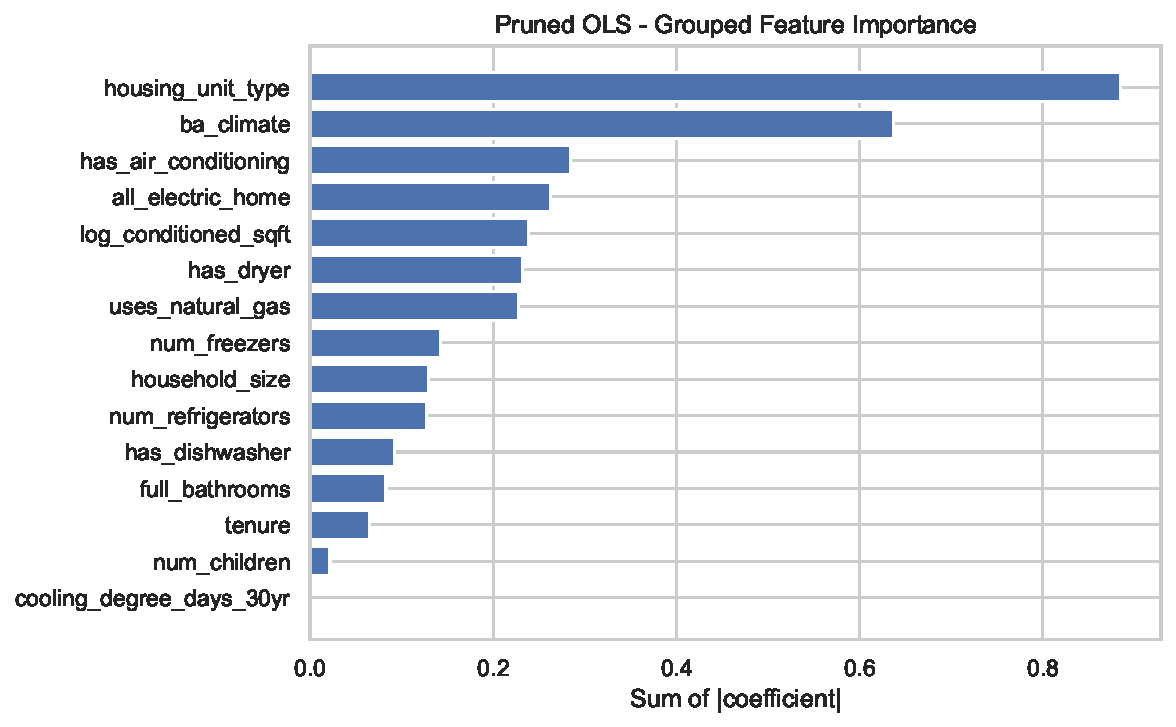
\includegraphics[width=\linewidth]{coefficient_importance_dot_plot.pdf}
\caption{Pruned OLS---grouped feature importance (sum of $|\beta|$).}
\label{fig:coef_imp}
\end{figure}

\subsection{Residual Diagnostics}

The residuals-vs-fitted plot (Figure~\ref{fig:resid}, left) shows approximately symmetric scatter with no strong curvilinear pattern, though variance increases slightly at higher fitted values. The QQ plot (right) reveals left-tail heaviness, consistent with the $-0.44$ skew in the log target.

Formal diagnostic tests (Table~\ref{tab:diag}) confirm non-normality (Jarque-Bera = 7{,}296, $p \approx 0$; kurtosis 6.23) and heteroskedasticity (Breusch-Pagan LM = 309, $p < 10^{-50}$). These justify the use of HC3 robust standard errors. Durbin-Watson of 2.05 indicates no serial autocorrelation.

\begin{table}[H]
\centering
\caption{Residual diagnostic tests---pruned OLS.}
\label{tab:diag}
\small
\begin{tabular}{@{}lrl@{}}
\toprule
\textbf{Test} & \textbf{Statistic} & \textbf{$p$-value}\\
\midrule
Jarque-Bera     & 7{,}296 & $\approx 0$ \\
Kolmogorov-Smirnov & 0.029 & 0.001 \\
Breusch-Pagan LM & 309.1  & $8.97\times10^{-51}$ \\
Breusch-Pagan $F$ & 12.6  & $2.27\times10^{-51}$ \\
Durbin-Watson  & 2.048 & --- \\
\bottomrule
\end{tabular}
\end{table}

\begin{figure}[H]
\centering
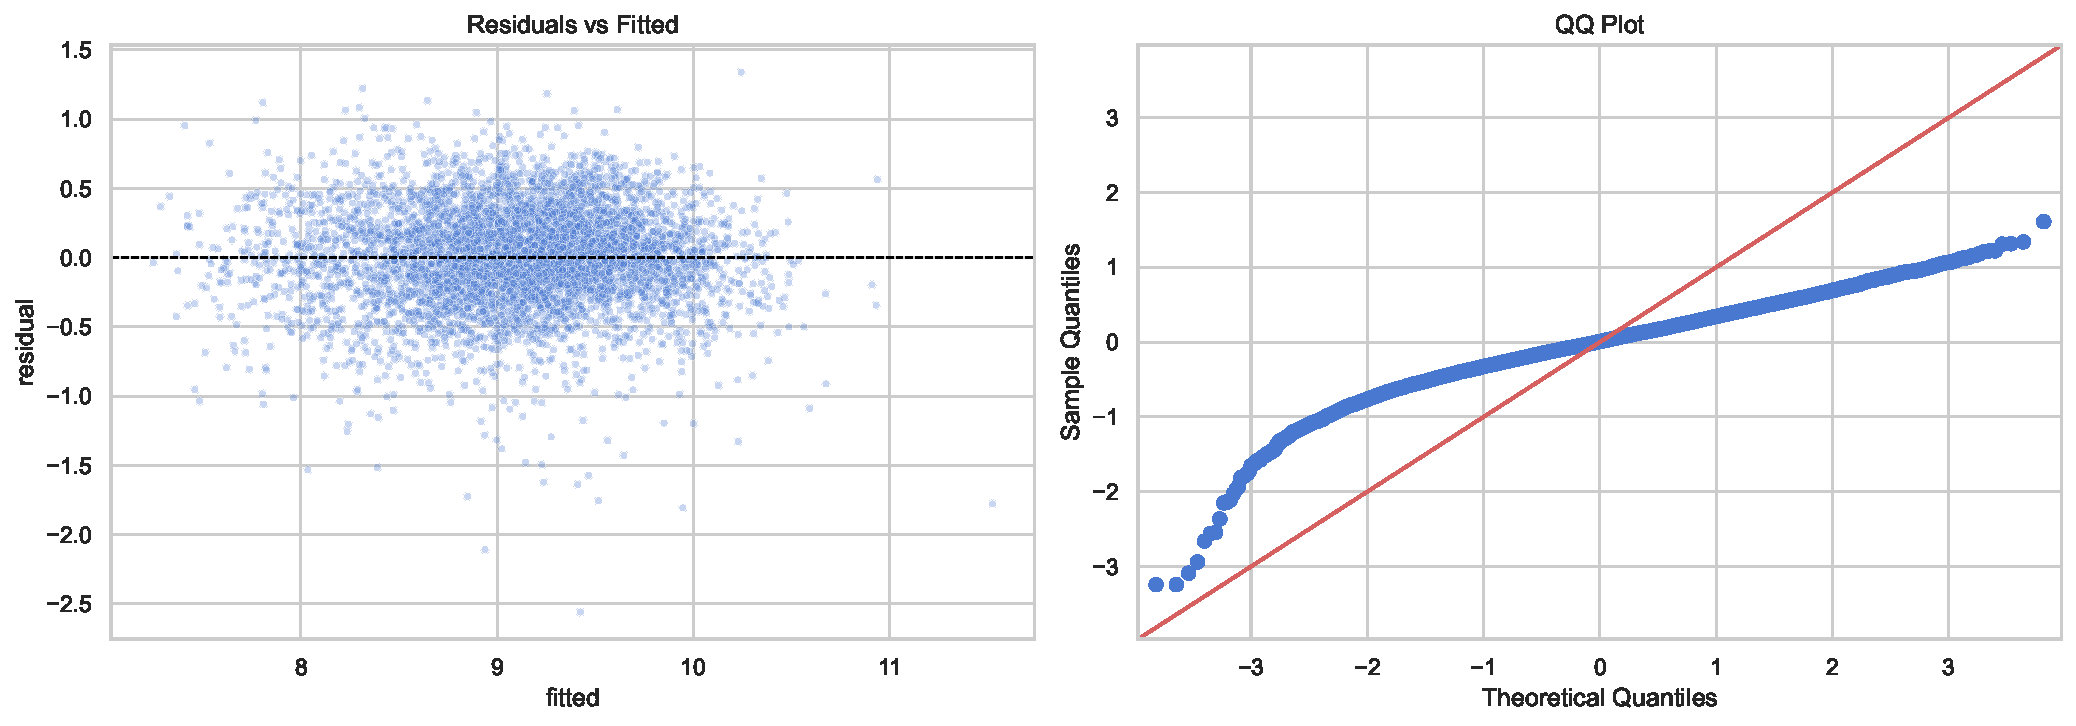
\includegraphics[width=\linewidth]{Residual_diagnostics.pdf}
\caption{Residuals vs.\ fitted (left) and QQ plot (right). Left-tail departure reflects residual skew; mild heteroskedasticity is addressed by HC3.}
\label{fig:resid}
\end{figure}

% ════════════════════════════════════════════════════════════
\section{Regularised and Tree-Based Models}

\subsection{Model Suite}

To benchmark OLS, we fit five additional model families on the expanded feature set (standardised numeric inputs):

\begin{itemize}
\item \textbf{Ridge} (RidgeCV, 25 $\alpha$ values from $10^{-3}$ to $10^3$)
\item \textbf{Lasso} (LassoCV, 5-fold CV, 20{,}000 max iterations)
\item \textbf{Elastic Net} (ElasticNetCV, $l_1$ ratios 0.1--1.0, 5-fold)
\item \textbf{PCA + Linear} (PCA at 95\% variance on numeric features, then OLS)
\item \textbf{HistGradientBoosting} (max depth 6, learning rate 0.05, 400 iterations)
\end{itemize}

All models except PCA were also run on the Engineered feature set to test whether derived features improve performance.

\subsection{Results}

Tables~\ref{tab:comparison_log} and~\ref{tab:comparison_kwh} present the full model comparison. Figure~\ref{fig:comparison} provides the visual summary.

\begin{table}[H]
\centering
\caption{Model comparison---log1p(KWH) scale.}
\label{tab:comparison_log}
\small
\setlength{\tabcolsep}{3pt}
\begin{tabular}{@{}lccccc@{}}
\toprule
\textbf{Model} & \textbf{Tr.} & \textbf{Te.} & \textbf{Te.} & \textbf{Te.} & \textbf{Te.}\\
               & $R^2$ & $R^2$ & RMSE & MAE & MAPE\\
\midrule
Eng.\ HGB         & .803 & .771 & .317 & .240 & 2.68\%\\
HGB                & .783 & .761 & .324 & .246 & 2.76\%\\
Eng.\ Linear       & .715 & .710 & .357 & .272 & 3.04\%\\
Eng.\ Ridge        & .715 & .710 & .357 & .272 & 3.04\%\\
Eng.\ Lasso        & .715 & .709 & .358 & .272 & 3.04\%\\
Eng.\ E-Net        & .715 & .709 & .358 & .272 & 3.04\%\\
Initial OLS        & .708 & .703 & .362 & .274 & 3.07\%\\
Pruned OLS         & .705 & .699 & .364 & .277 & 3.10\%\\
Linear Reg.        & .705 & .699 & .364 & .277 & 3.10\%\\
Ridge              & .705 & .699 & .364 & .277 & 3.10\%\\
Lasso              & .705 & .699 & .364 & .277 & 3.10\%\\
Elastic Net        & .705 & .699 & .364 & .277 & 3.10\%\\
PCA + Lin.         & .698 & .691 & .369 & .280 & 3.14\%\\
Naive Baseline     & .000 & $-$.001 & .663 & .530 & 5.98\%\\
\bottomrule
\end{tabular}
\end{table}

\begin{table}[H]
\centering
\caption{Model comparison---KWH scale (business view).}
\label{tab:comparison_kwh}
\small
\setlength{\tabcolsep}{3pt}
\begin{tabular}{@{}lccccc@{}}
\toprule
\textbf{Model} & \textbf{Tr.} & \textbf{Te.} & \textbf{Te.} & \textbf{Te.} & \textbf{Te.}\\
               & $R^2$ & $R^2$ & RMSE & MAE & MAPE\\
\midrule
Eng.\ HGB         & .766 & .719 & 3{,}597 & 2{,}402 & 25.7\%\\
HGB                & .735 & .714 & 3{,}630 & 2{,}464 & 26.6\%\\
Eng.\ Linear       & .605 & .599 & 4{,}302 & 2{,}783 & 29.7\%\\
Eng.\ Ridge        & .605 & .599 & 4{,}302 & 2{,}782 & 29.7\%\\
Initial OLS        & .601 & .600 & 4{,}298 & 2{,}797 & 30.2\%\\
Pruned OLS         & .595 & .590 & 4{,}347 & 2{,}828 & 30.5\%\\
Ridge              & .596 & .591 & 4{,}346 & 2{,}827 & 30.5\%\\
Lasso              & .596 & .591 & 4{,}345 & 2{,}827 & 30.5\%\\
PCA + Lin.         & .595 & .576 & 4{,}422 & 2{,}853 & 31.0\%\\
Naive              & $-$.080 & $-$.071 & 7{,}028 & 5{,}074 & 66.3\%\\
\bottomrule
\end{tabular}
\end{table}

\begin{figure}[H]
\centering
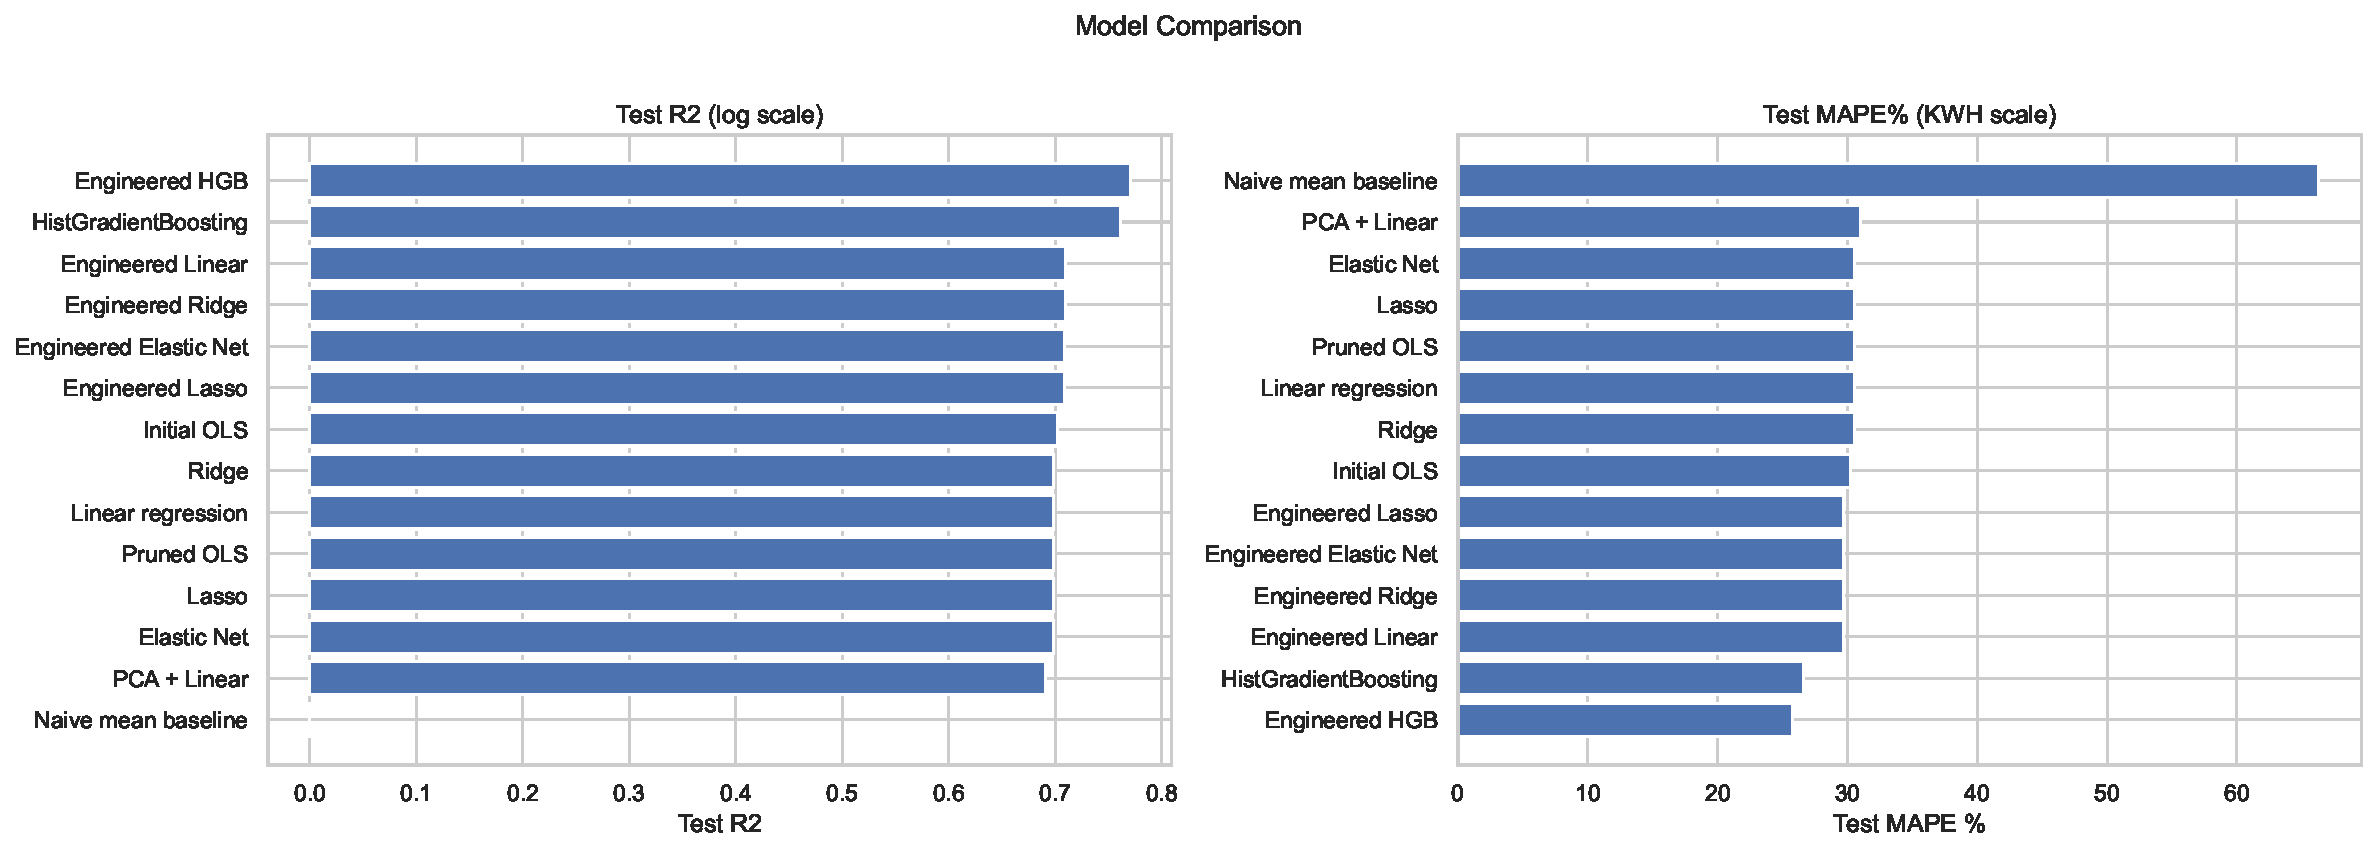
\includegraphics[width=\linewidth]{test_R2_and_test_MAPE.pdf}
\caption{Test $R^2$ on log scale (left) and test MAPE on KWH scale (right). Gradient boosting models clearly separate from the linear cluster.}
\label{fig:comparison}
\end{figure}

\subsection{Analysis of Results}

\textbf{Linear models are tightly clustered.} Pruned OLS, sklearn Linear Regression, Ridge, Lasso, and Elastic Net all achieve test $R^2 \approx 0.699$ on the log scale and ${\sim}0.59$ on KWH. Regularisation provides no meaningful lift, confirming that the VIF-pruned OLS specification is already near-efficient with no significant overfitting to regularise away. This is a notable finding: it demonstrates that careful feature selection via VIF diagnostics can be as effective as automated regularisation.

\textbf{Engineered features add consistent signal.} The engineered set lifts linear models from $R^2 = 0.699$ to $0.710$ (+1.1~pp), driven by \texttt{electronics\_load\_proxy} and \texttt{ac\_unit\_count}. This gain is consistent across all linear model families, suggesting the composites capture real aggregated-device effects that individual appliance counts cannot represent as efficiently.

\textbf{HistGradientBoosting captures nonlinearities.} HGB achieves test $R^2 = 0.761$ (expanded) and $0.771$ (engineered)---a 6--7~pp lift over linear models. On KWH scale: $R^2 = 0.714$--$0.719$ vs.\ ${\sim}0.59$ for linear models. The train-test gap for Engineered HGB is 0.803 vs.\ 0.771 (3.2~pp), indicating moderate but acceptable overfitting given the model's complexity. This performance gap implies interaction effects (climate $\times$ AC, size $\times$ occupancy) and nonlinear thresholds that additive models cannot represent. For example, the marginal effect of an additional AC unit likely depends on climate zone---a relationship HGB captures automatically through its tree splits.

\textbf{PCA + Linear underperforms.} Compressing numeric features to principal components sacrifices ${\sim}1$~pp in $R^2$, indicating that individual features carry axis-aligned signals that PCA rotation obscures.

\textbf{Log-to-KWH retransformation gap.} A consistent pattern across all models is that $R^2$ drops substantially when converting from log to KWH scale (e.g., Pruned OLS goes from 0.699 to 0.590). This is expected: the $\text{expm1}(\cdot)$ back-transformation amplifies errors for high-consumption households. Additionally, Jensen's inequality means that $E[\exp(\hat{y})] \neq \exp(E[\hat{y}])$, introducing a systematic negative bias. A Duan smearing estimator could correct this, but was not applied here since our focus is on relative model comparison rather than point forecasting.

\textbf{Naive baseline context.} The naive mean baseline achieves $R^2 = -0.001$ on log scale and $-0.071$ on KWH scale. The negative KWH-scale $R^2$ confirms that predicting the log-scale mean and exponentiating is worse than predicting the raw-scale mean directly, due to the Jensen's inequality bias. All fitted models improve massively over this floor.

\subsection{Cross-Model Feature Importance}

Feature rankings are remarkably stable across Pruned OLS, Linear Regression, Ridge, and Lasso (Figure~\ref{fig:grouped}): \texttt{housing\_unit\_type} and \texttt{ba\_climate} dominate in all four, followed by \texttt{has\_air\_conditioning}, \texttt{all\_electric\_home}, and \texttt{has\_dryer}. This consistency validates the robustness of the core feature set.

\begin{figure}[H]
\centering
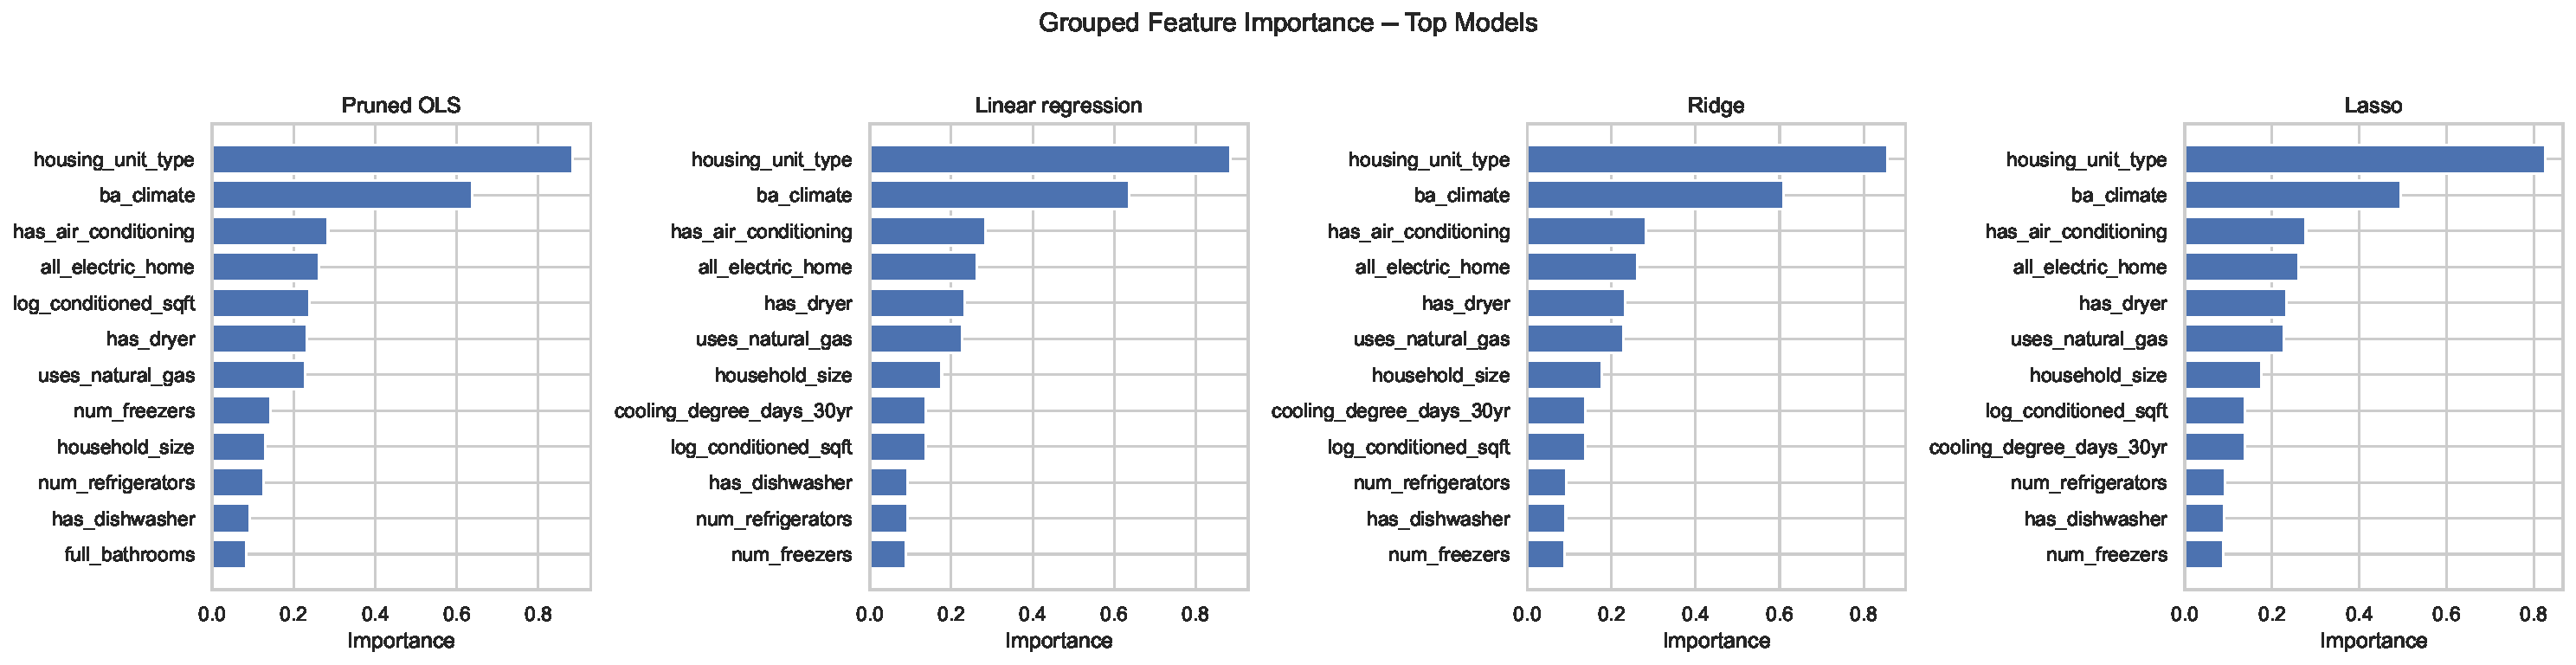
\includegraphics[width=\linewidth]{Grouped_importance.pdf}
\caption{Grouped feature importance across top linear models. Rankings are stable; magnitudes differ due to standardisation (OLS uses raw-scale; regularised models use standardised inputs).}
\label{fig:grouped}
\end{figure}

% ════════════════════════════════════════════════════════════
\section{Discussion}

\subsection{Coefficient Interpretation}

Since the dependent variable is $\log(1 + \text{KWH})$, each coefficient approximates a percentage change in KWH per unit increase (for $|\beta| < 0.2$; larger effects require exponentiation):

\begin{itemize}
\item A 1\% increase in conditioned sqft $\Rightarrow$ ${\sim}0.24\%$ higher annual KWH (log-log elasticity).
\item Air conditioning adds ${\sim}33\%$ ($e^{0.284} - 1$).
\item All-electric homes use ${\sim}30\%$ more ($e^{0.263} - 1$); natural gas access reduces electricity by ${\sim}20\%$ ($1 - e^{-0.227}$)---fuel substitution.
\item Each additional member adds ${\sim}14\%$; children contribute less (net $+11\%$ per child vs.\ $+14\%$ per adult).
\item Mobile homes consume ${\sim}49\%$ more ($e^{0.399} - 1$) than the Apartment 2--4 reference.
\end{itemize}

\subsection{Limitations}

\textbf{Heteroskedasticity.} Despite log transformation, Breusch-Pagan rejects homoskedasticity ($p < 10^{-50}$). HC3 SEs correct inference but do not improve prediction intervals.

\textbf{Residual non-normality.} Kurtosis of 6.23 (vs.\ normal 3.0) means normality-based prediction intervals would be miscalibrated, though coefficient $p$-values are asymptotically valid at $n = 14{,}796$.

\textbf{Unweighted estimation.} RECS uses a complex survey design. Population-level inference requires survey weights and strata. Our sample-conditional estimates may differ from population-average effects.

\textbf{Single split.} An 80/20 split provides point estimates without uncertainty on comparison metrics. Cross-validation was used for regularisation hyperparameters but not for final $R^2$ variance estimation.

\textbf{Omitted variables.} Electricity prices, insulation quality, HVAC efficiency ratings, and detailed behavioural patterns beyond thermostat settings are plausibly important but absent from or excluded from our feature set.

\subsection{Practical Implications}

The results carry several implications for energy policy and utility planning:

\textbf{Targeting high-consumption segments.} The OLS model identifies mobile homes in hot-humid climates as the highest-consuming segment. Weatherisation and insulation retrofit programmes targeting this segment would yield the largest per-household savings.

\textbf{All-electric transition.} The 30\% electricity premium for all-electric homes (controlling for other factors) quantifies the grid-level impact of fuel switching. As gas heating is phased out, utilities should anticipate a proportional increase in peak electricity demand concentrated in winter months.

\textbf{Appliance and electronics load.} The significance of \texttt{num\_freezers}, \texttt{num\_refrigerators}, and the \texttt{electronics\_load\_proxy} suggests that appliance efficiency standards and electronics power management remain relevant policy levers. Each additional freezer adds ${\sim}15\%$ to annual consumption.

\textbf{Limits of behavioural interventions.} The weak univariate signal from thermostat setpoints (Figure~\ref{fig:thermo}) and the dominance of structural features in the OLS suggest that nudge-based interventions (e.g., smart thermostat programmes) will have smaller effects than structural measures (insulation, HVAC upgrades, building codes).

\subsection{Model Selection Guidance}

For \textit{interpretability} (e.g., regulatory filings, policy reports), the pruned OLS with HC3 remains the recommended model. Its coefficients are directly interpretable, all $p$-values are reported with robust standard errors, and the model is fully transparent.

For \textit{prediction} (e.g., demand forecasting, customer segmentation), HistGradientBoosting on the engineered feature set is preferred, offering $R^2 = 0.77$ on log scale with a test MAPE of ${\sim}26\%$ on KWH---a substantial improvement over linear models' ${\sim}30\%$.

% ════════════════════════════════════════════════════════════
\section{Conclusion}

This analysis demonstrates that a compact set of dwelling, equipment, occupancy, and climate features explains ${\sim}70\%$ of the log-variance in U.S.\ household annual electricity consumption. The pruned OLS model (test $R^2 = 0.699$) with HC3 robust standard errors identifies housing type, climate zone, air conditioning, all-electric status, dwelling size, and dryer ownership as the dominant drivers.

Regularised linear models match OLS closely, confirming the specification is near-efficient for linear methods. HistGradientBoosting delivers a meaningful lift to test $R^2 \approx 0.77$ on log scale (0.72 on KWH), indicating nonlinearities and interactions that linear models miss. The engineered feature set adds ${\sim}1$~pp to linear models and yields the best HGB result (0.77), validating that composite features capture real incremental signal.

For practitioners, the key insight is that household electricity consumption is primarily a \textit{structural and geographic} phenomenon: the type, size, and climate zone of a dwelling, combined with its fuel source, explain the majority of variance. Behavioural factors---thermostat settings, appliance usage patterns, lighting habits---contribute at the margin but are secondary to these structural determinants.

\subsection*{Future Work}

Several extensions could strengthen this analysis. First, incorporating survey weights via weighted least squares would yield population-representative coefficient estimates. Second, interaction terms (e.g., climate $\times$ AC status, housing type $\times$ all-electric) could partially close the gap between OLS and HGB without sacrificing interpretability. Third, electricity price data (available at the state level from EIA) could be merged to test price elasticity of demand. Finally, the 2020 survey coincides with COVID-19 stay-at-home orders; a comparison with the forthcoming 2025 RECS wave would reveal whether the at-home effect on electricity use was transient or persistent.

% ════════════════════════════════════════════════════════════
\section*{References}

\begin{enumerate}[label={[\arabic*]},leftmargin=1.5em,nosep]
\item U.S.\ Energy Information Administration, ``2020 Residential Energy Consumption Survey (RECS) Microdata,'' 2023. \url{https://www.eia.gov/consumption/residential/data/2020/}
\item White, H. (1980). ``A heteroskedasticity-consistent covariance matrix estimator and a direct test for heteroskedasticity.'' \textit{Econometrica}, 48(4), 817--838.
\item Tibshirani, R. (1996). ``Regression shrinkage and selection via the lasso.'' \textit{J.\ Royal Statistical Society B}, 58(1), 267--288.
\item Ke, G.\ et al.\ (2017). ``LightGBM: A Highly Efficient Gradient Boosting Decision Tree.'' \textit{NeurIPS}.
\end{enumerate}

\end{document}